\subsection{Task 5.1 -- Hoàn thiện MVP}

Sprint 2 nối luồng xem menu với giỏ hàng, đặt đơn, thanh toán và nhận đồ tại
quầy. Web triển khai các màn hình chi tiết món, giỏ, xác thực, checkout và lịch
sử đơn. NestJS quản lý nghiệp vụ, trạng thái đơn và dữ liệu trong PostgreSQL.

\begin{enumerate}[leftmargin=*]
  \item \textbf{Chọn món và cập nhật giỏ.} Khách chọn size, topping phù hợp và
        số lượng. Giỏ cho sửa số lượng, xóa món và xem tổng tiền. Web hiển
        thị tiền tạm tính và giảm giá. API kiểm tra lại giá, tùy chọn và tồn
        khả dụng trước khi chấp nhận đơn.
  \item \textbf{Xác thực và tạo đơn.} Khách đăng ký, xác minh email bằng OTP
        và đăng nhập. API dùng JWT để bảo vệ thao tác đặt hàng và kiểm tra
        quyền truy cập đơn. Đơn mới có trạng thái \texttt{PENDING}. API giữ
        nguyên liệu theo công thức trong thời hạn 120 giây.
  \item \textbf{Thanh toán.} Kênh CARD dùng cổng mô phỏng. Lựa chọn ví/QR
        dùng VietQR qua PayOS khi có cấu hình. Bộ test có thể giả lập kết quả
        PayOS bằng link và webhook ký bằng khóa thử. API dùng khóa giao
        dịch và kiểm tra trạng thái đơn để tránh ghi nhận trùng. Thanh toán
        thành công chuyển đơn sang \texttt{PAID} và tiêu thụ nguyên liệu đã giữ.
  \item \textbf{Xác nhận và theo dõi.} Khách xem biên nhận, trạng thái hiện
        tại và lịch sử đơn. Nhân viên xử lý các bước pha chế, sẵn sàng và hoàn
        tất trên giao diện quản trị.
  \item \textbf{Xử lý lỗi.} Web hiển thị lỗi nhập liệu, thiếu nguyên liệu hoặc
        lỗi thanh toán. API kiểm tra DTO, quyền truy cập, trạng thái đơn và
        dữ liệu giao dịch. Khi đơn QR hết hạn, API đối soát với PayOS trước
        khi quyết định hủy và trả phần nguyên liệu đã giữ.
\end{enumerate}

Chi tiết luồng thành công và ngoại lệ nằm ở UC-01. Bộ kiểm thử liên quan được
liệt kê ở Task 5.2 và \nolinkurl{tests/README.md}.

\paragraph{Minh chứng giỏ hàng, voucher và checkout}
Các ảnh Sprint 2 được chụp ngày 20/11/2026 trên môi trường demo local,
dùng DB \nolinkurl{brewlite_report} và tài khoản thử đã xác minh email.
Khách chọn một Bạc Xỉu size M giá 39.000đ, áp mã \texttt{WELCOME10} giảm
3.900đ, còn thanh toán 35.100đ. Giao dịch dùng kênh CARD mô phỏng.

Ảnh chụp vùng nội dung checkout hiển thị đúng món, voucher, tổng tiền và
điểm dự kiến. Thẻ điền sẵn là dữ liệu mô phỏng. Kênh PayOS thật không được
cấu hình trong môi trường demo local này; ảnh không chứng minh một giao
dịch ngân hàng hoặc VietQR thật.

\begin{reportfigure}
\begin{minipage}{.78\linewidth}
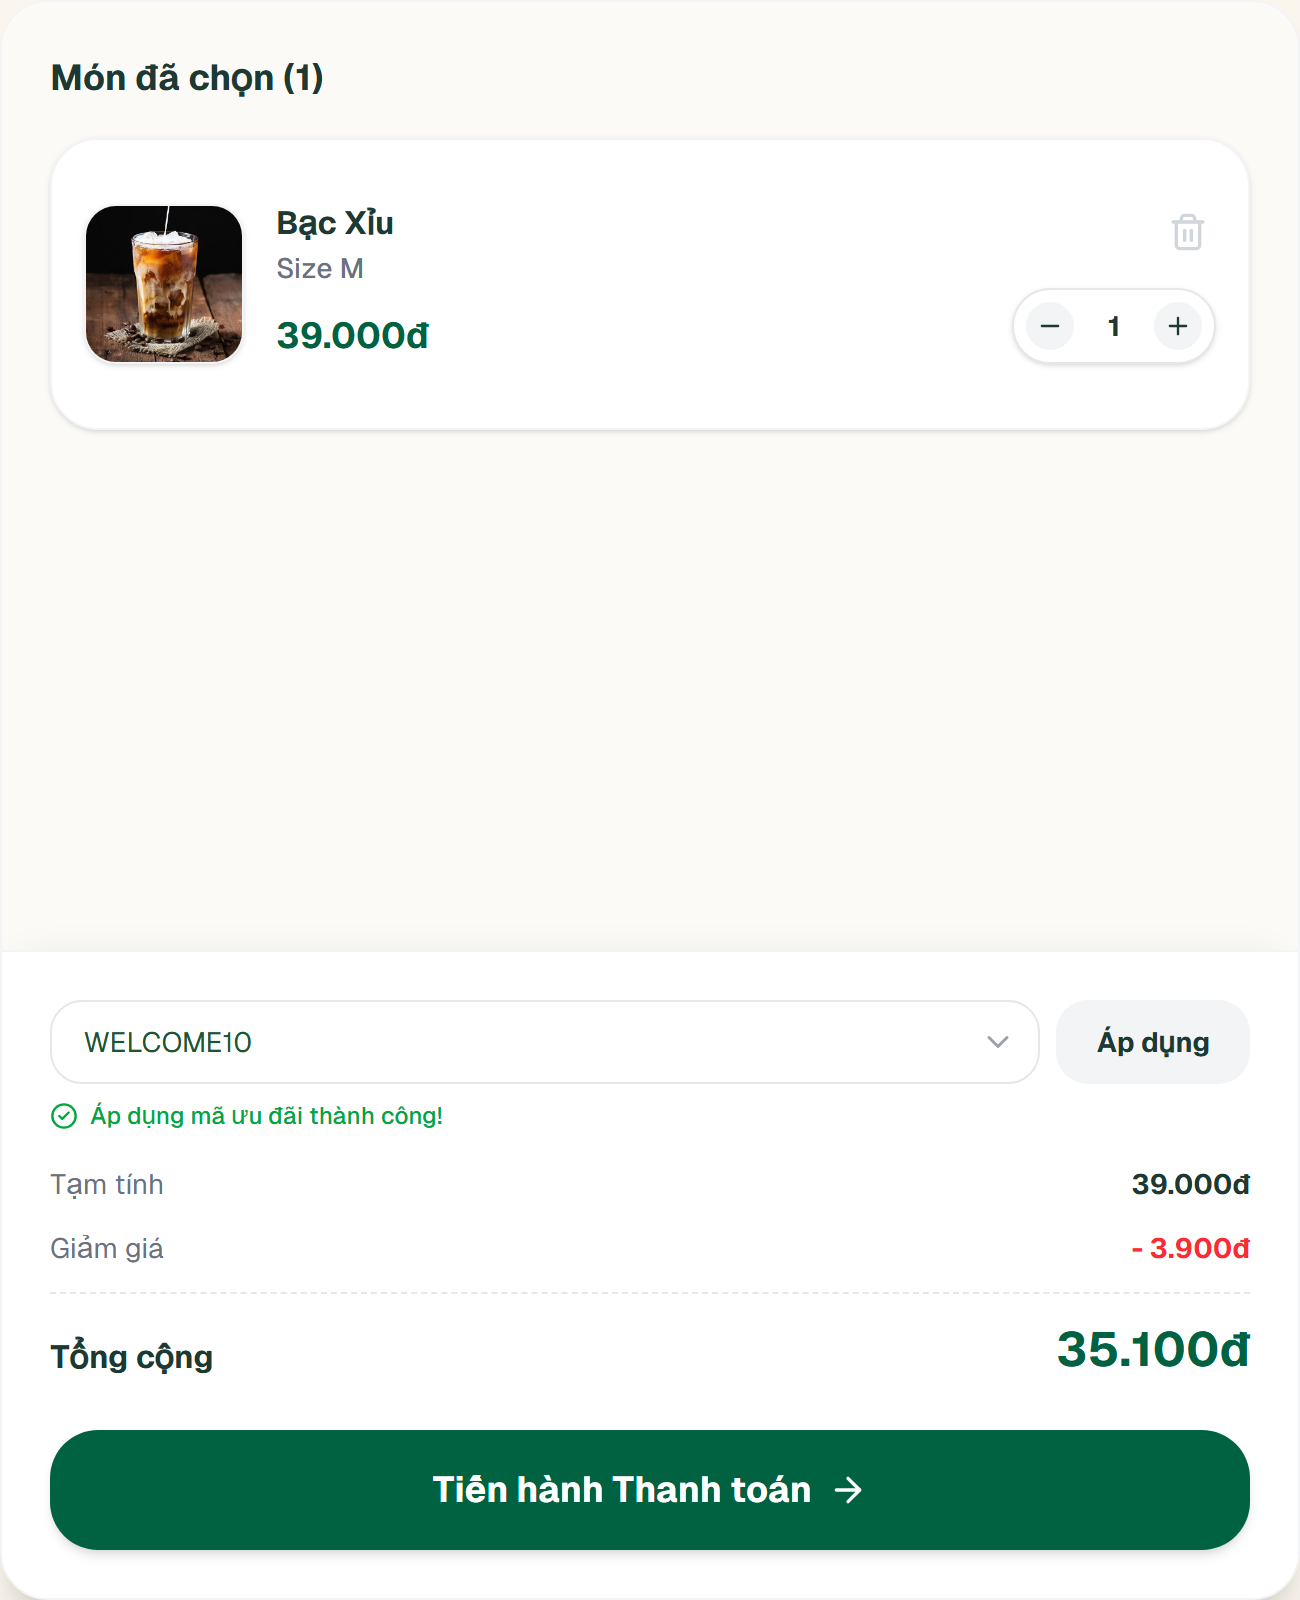
\includegraphics[width=\linewidth,trim=0bp 1160bp 0bp 0bp,clip]{../../assets/evidence/sprint2-cart.png}\\[3pt]
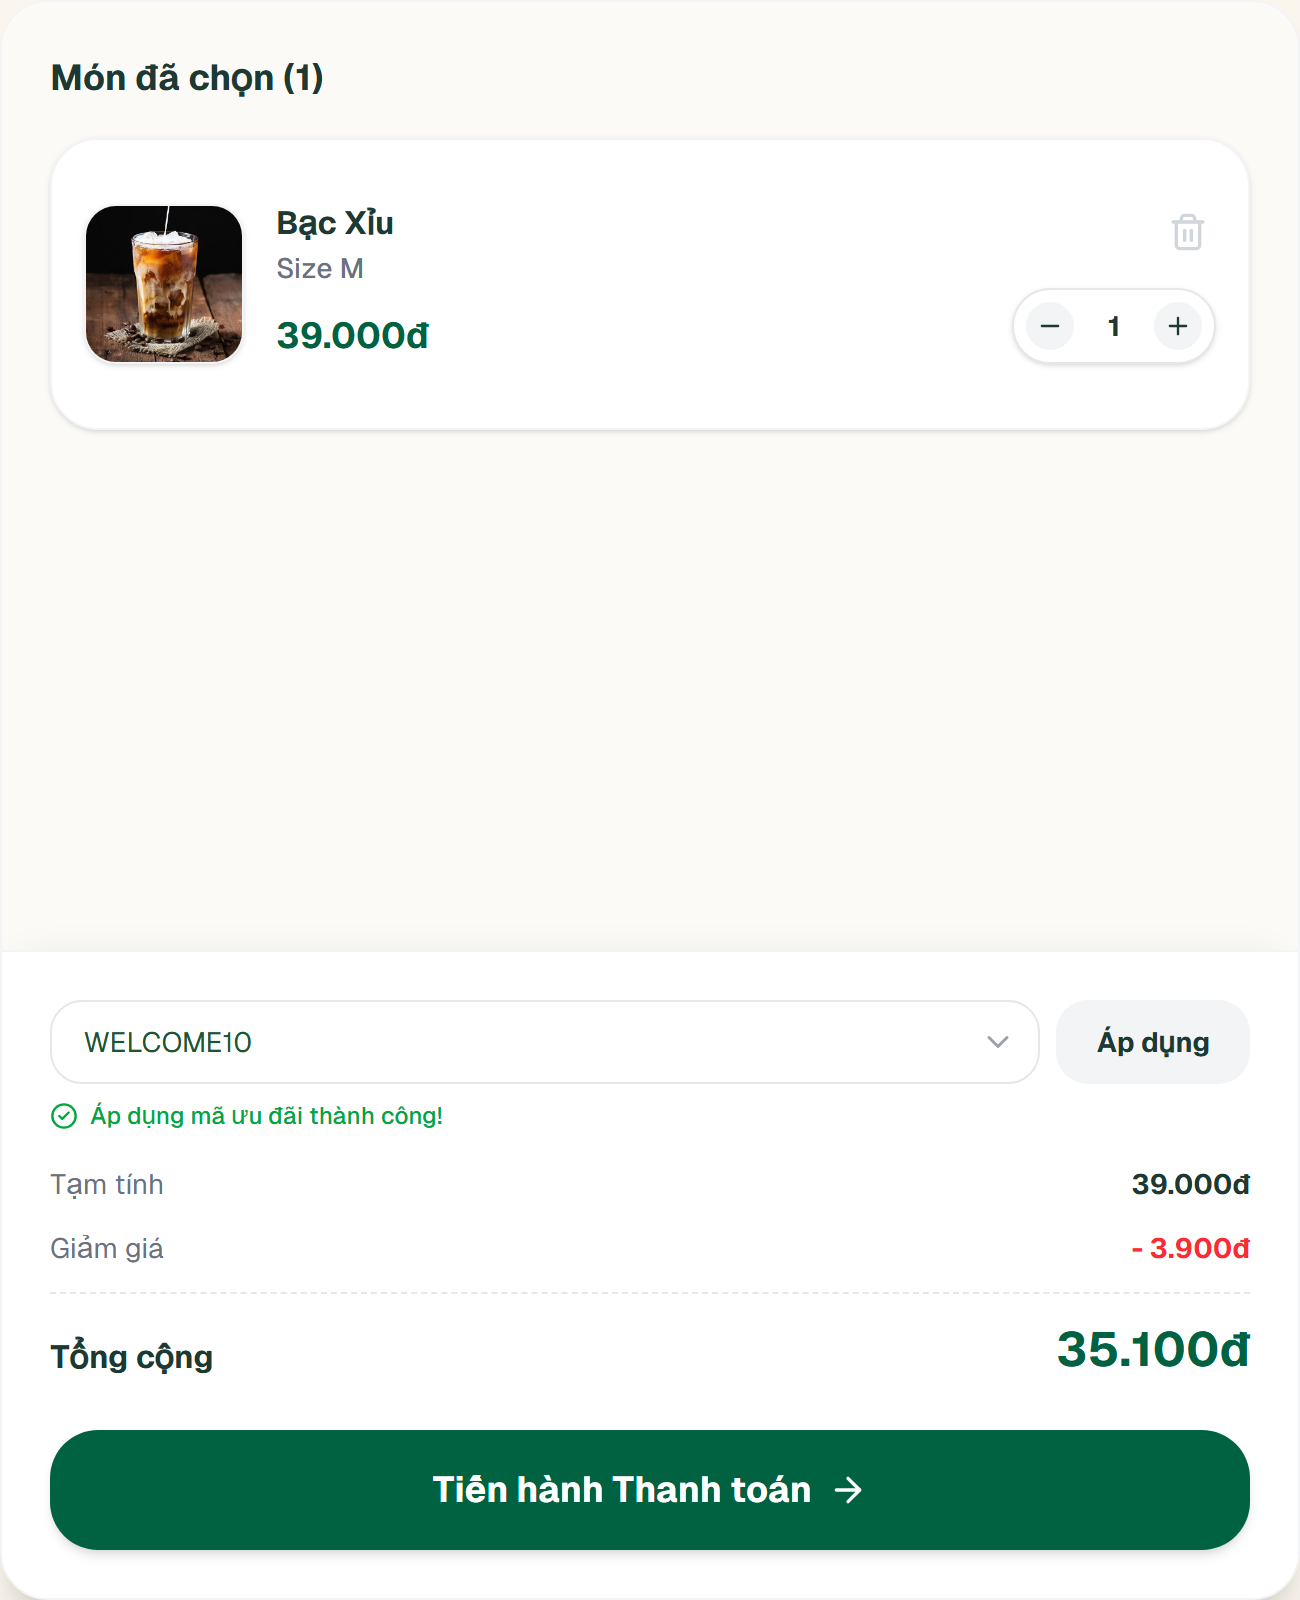
\includegraphics[width=\linewidth,trim=0bp 0bp 0bp 950bp,clip]{../../assets/evidence/sprint2-cart.png}
\end{minipage}
\par\small\itshape Hình 5.1a. Trích vùng món đã chọn và tổng tiền sau voucher WELCOME10
\par\medskip\normalfont\normalsize
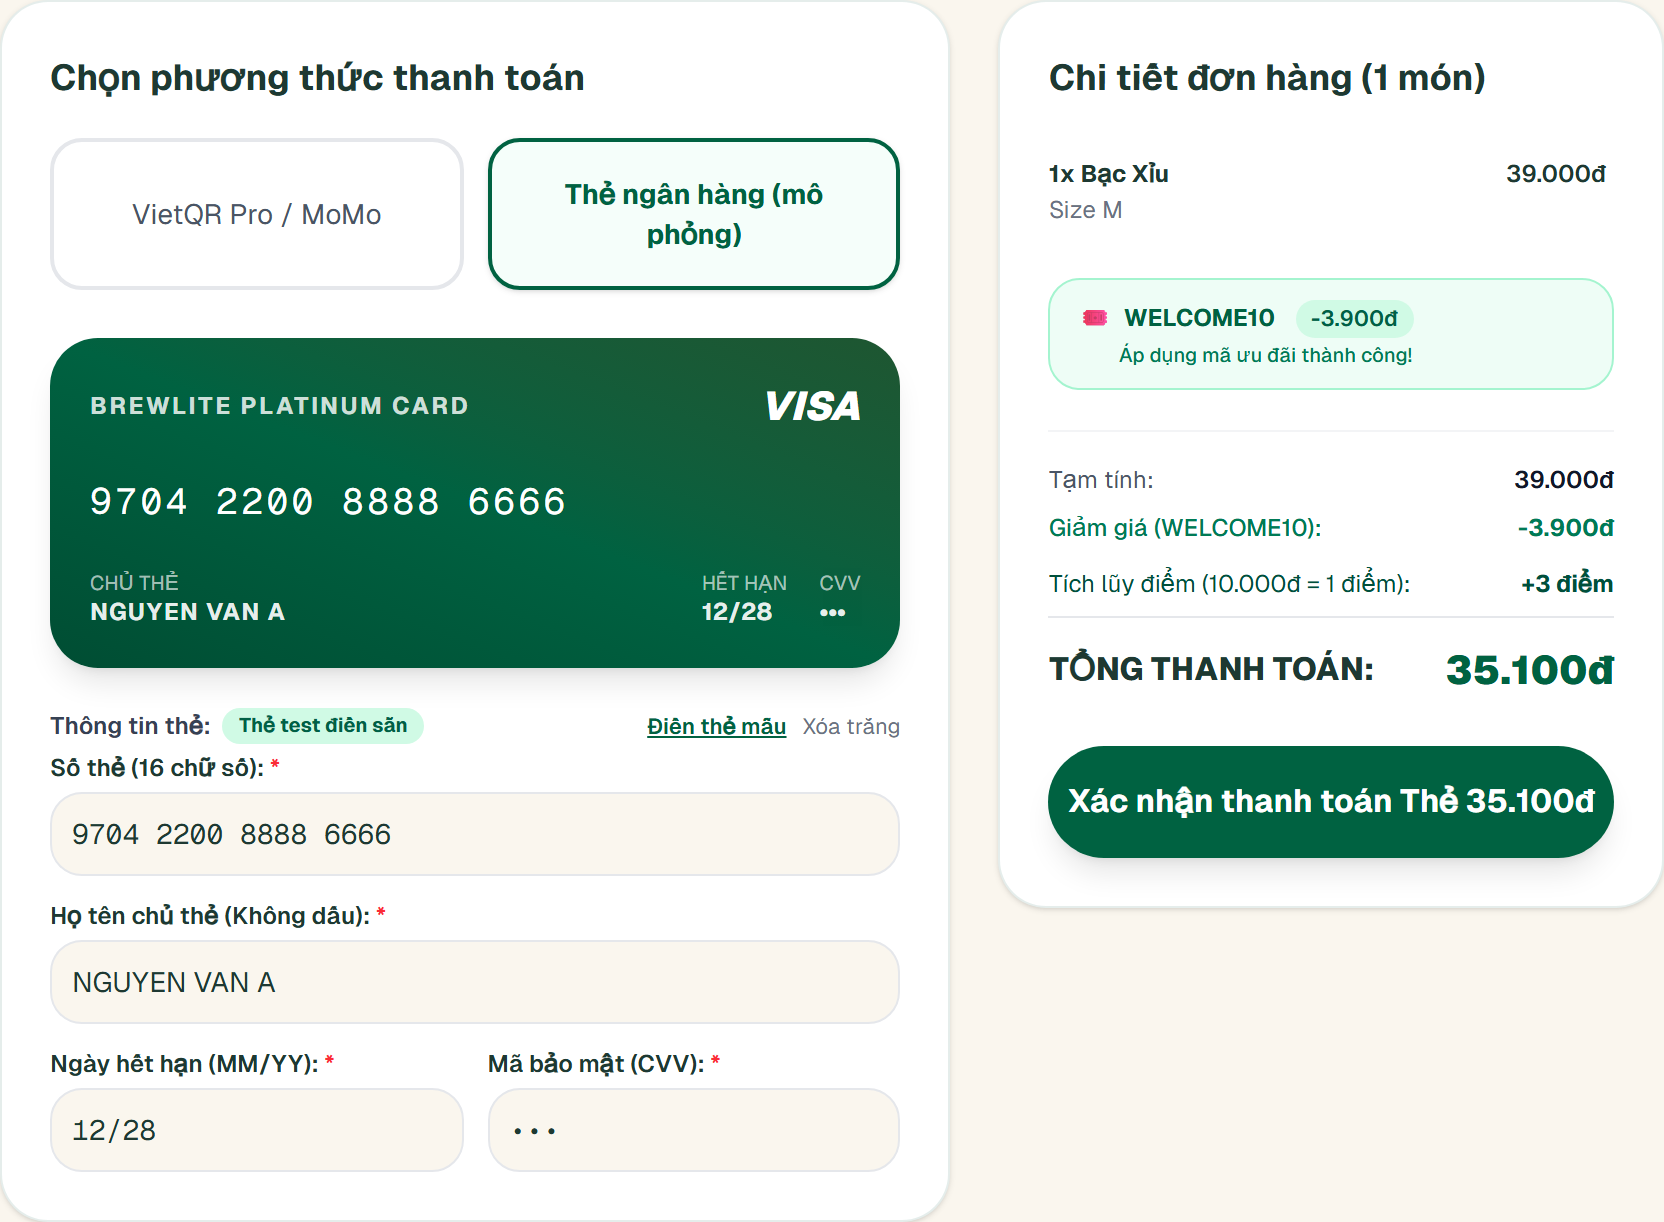
\includegraphics[width=\linewidth,height=.70\textheight,keepaspectratio]{../../assets/evidence/sprint2-checkout.png}
\par\small\itshape Hình 5.1b. Vùng phương thức thanh toán thẻ mô phỏng và tóm tắt đơn
\end{reportfigure}

\paragraph{Minh chứng biên nhận sau thanh toán}\leavevmode\par\nobreak
\begin{reportfigure}
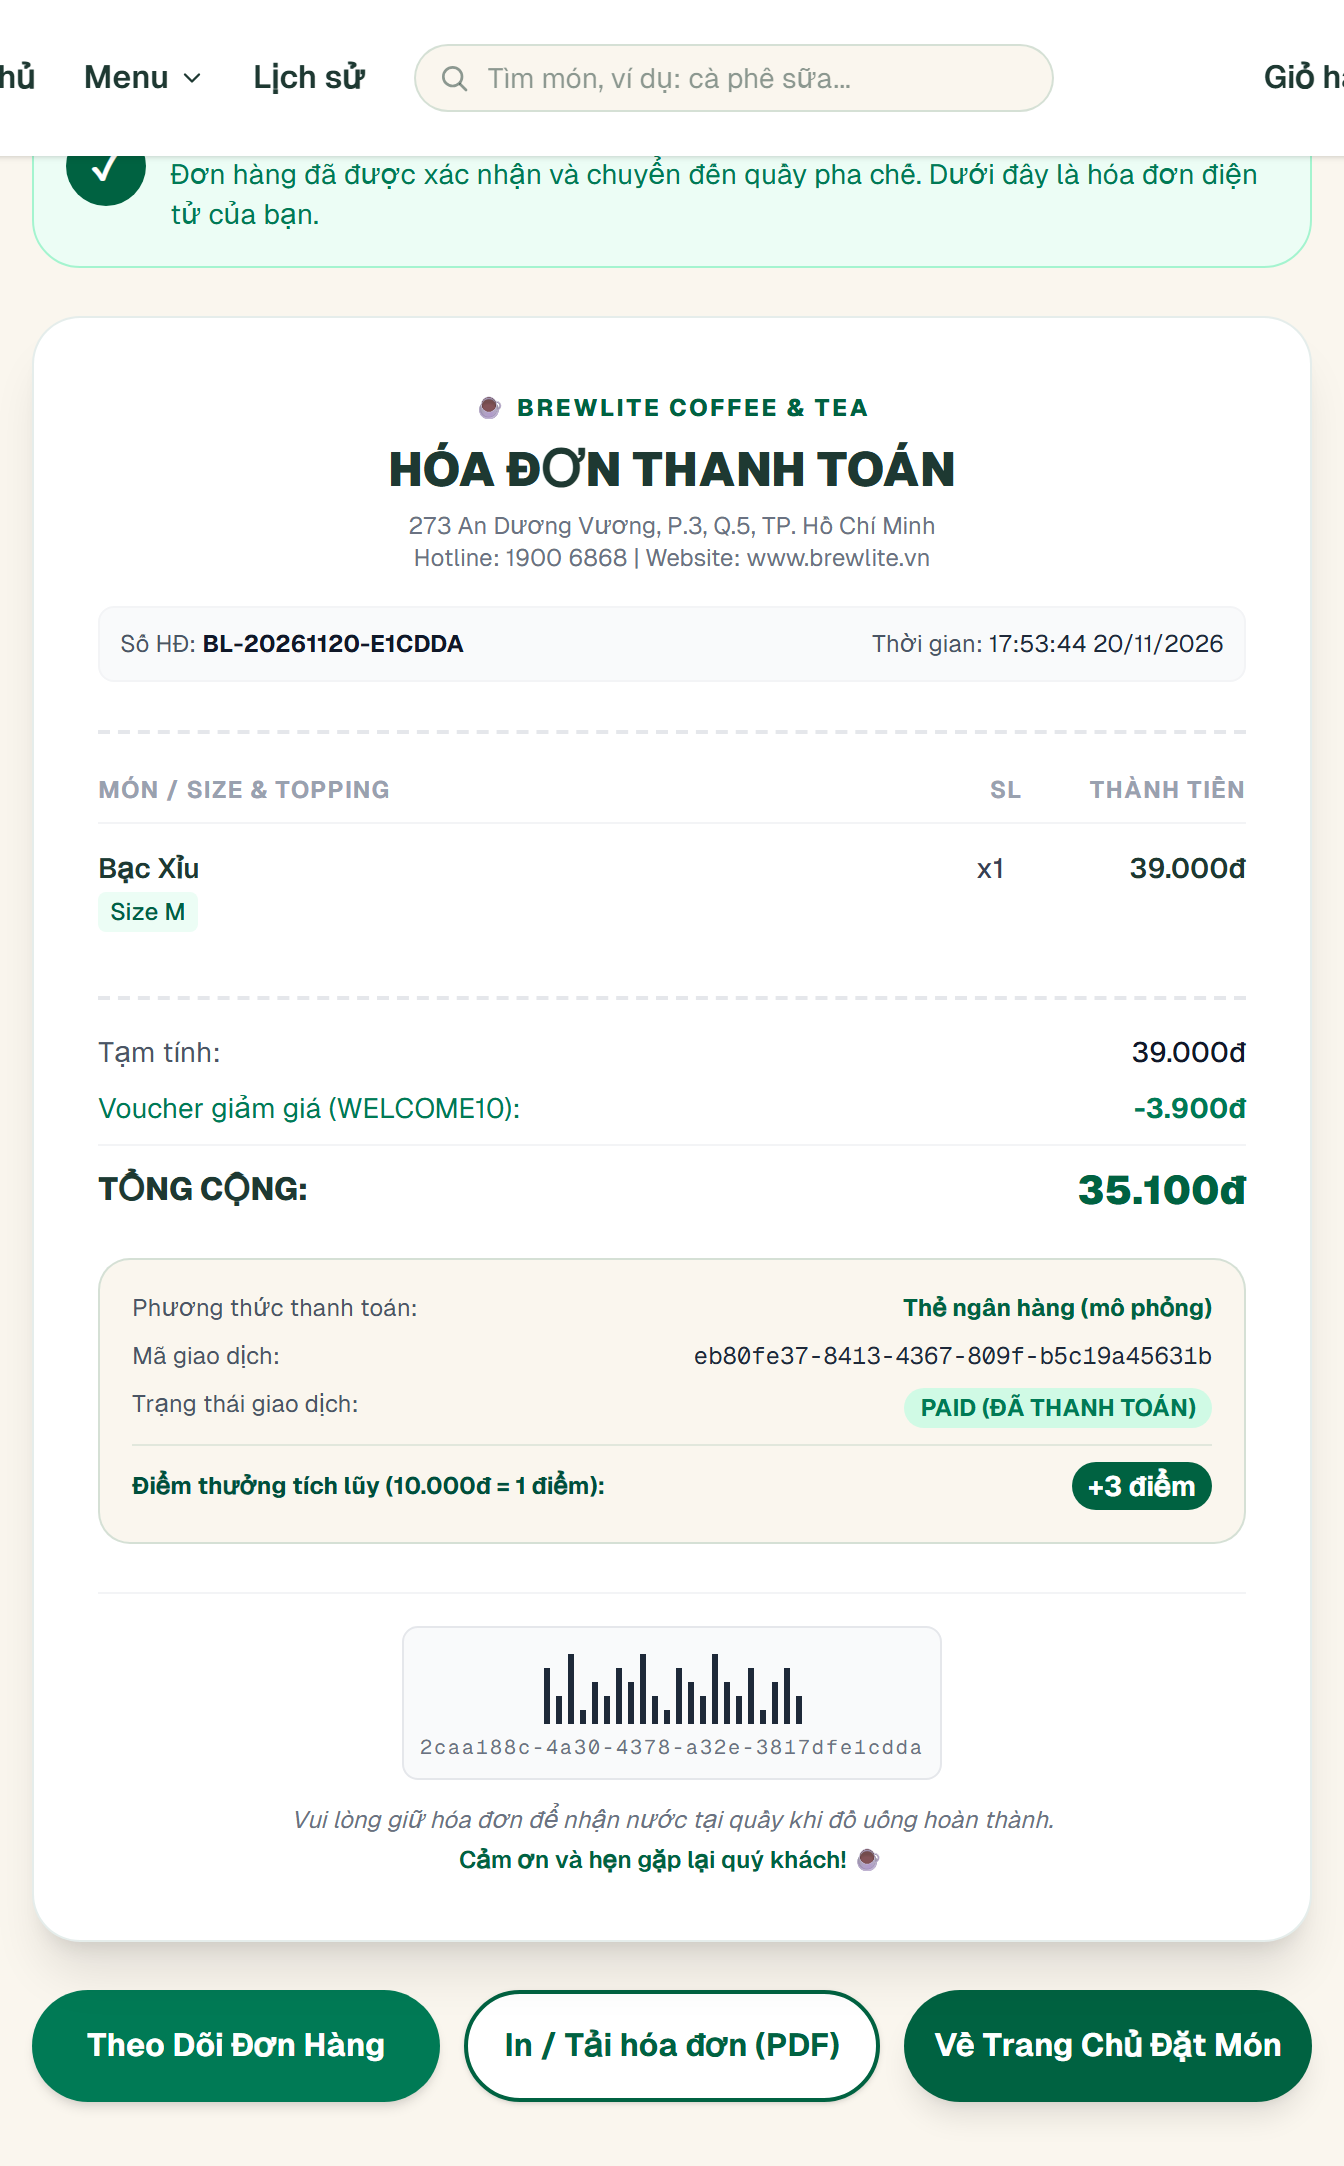
\includegraphics[width=.80\linewidth,height=.73\textheight,keepaspectratio,trim=0bp 0bp 0bp 300bp,clip]{../../assets/evidence/sprint2-receipt.png}
\par\small\itshape Hình 5.1c. Biên nhận CARD mô phỏng: PAID, tổng 35.100đ và cộng 3 điểm
\end{reportfigure}

API đã xác nhận thanh toán trước khi giao diện hiển thị hóa đơn. Mã đơn
được giữ để đối chiếu với màn hình theo dõi và lịch sử bên dưới.

\paragraph{Minh chứng theo dõi và lịch sử đơn}\leavevmode\par\nobreak
\begin{reportfigure}
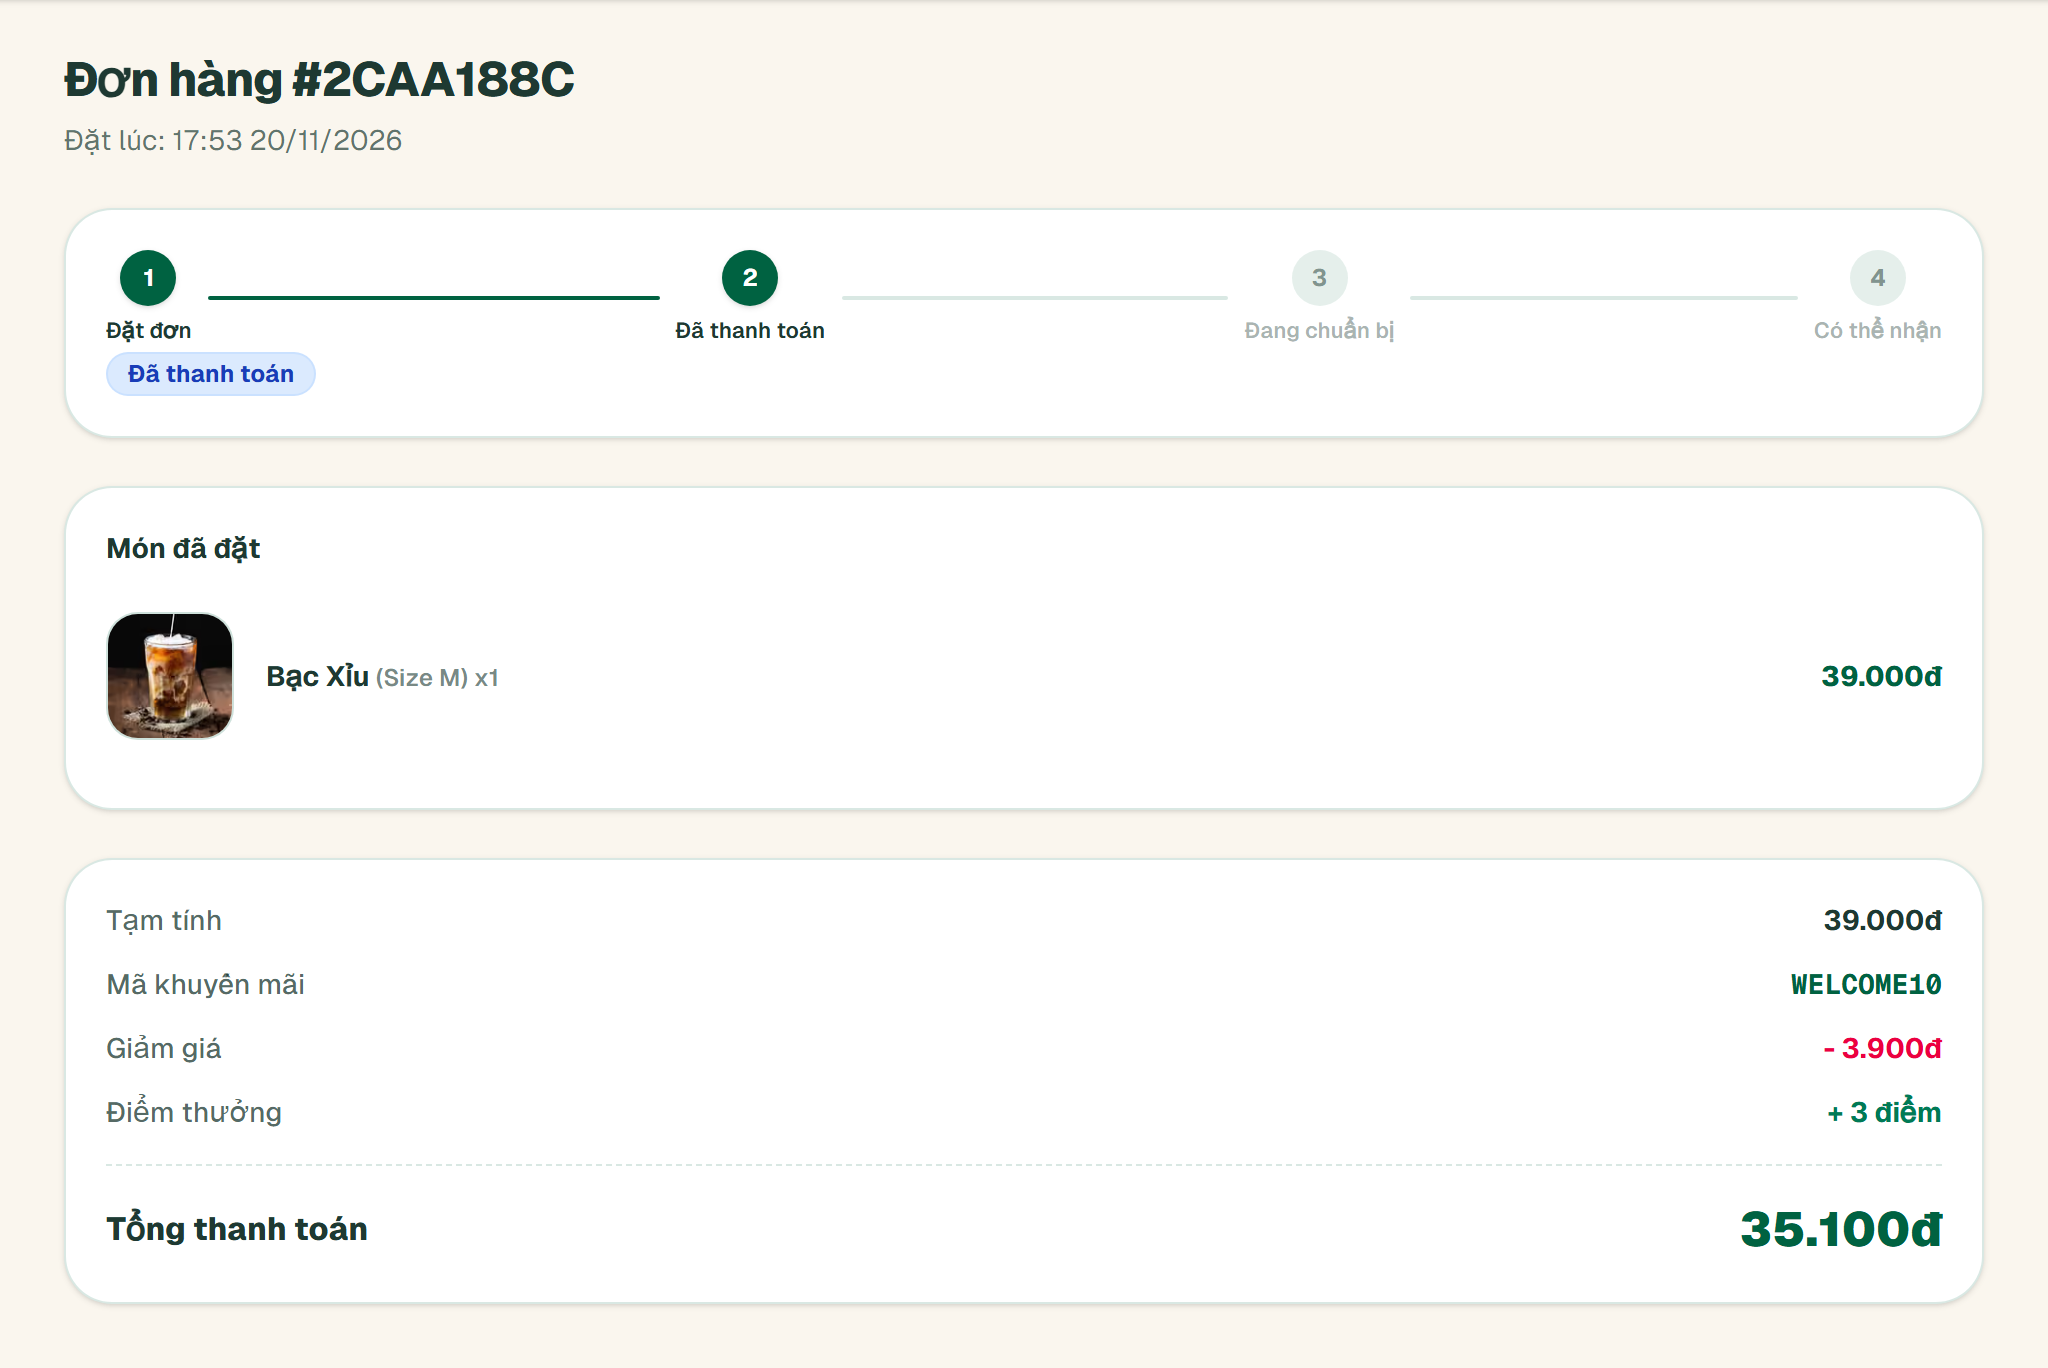
\includegraphics[width=\linewidth,height=.37\textheight,keepaspectratio]{../../assets/evidence/sprint2-order-detail.png}
\par\small\itshape Hình 5.1d. Chi tiết đơn sau thanh toán và tiến trình xử lý
\end{reportfigure}
\begin{reportfigure}
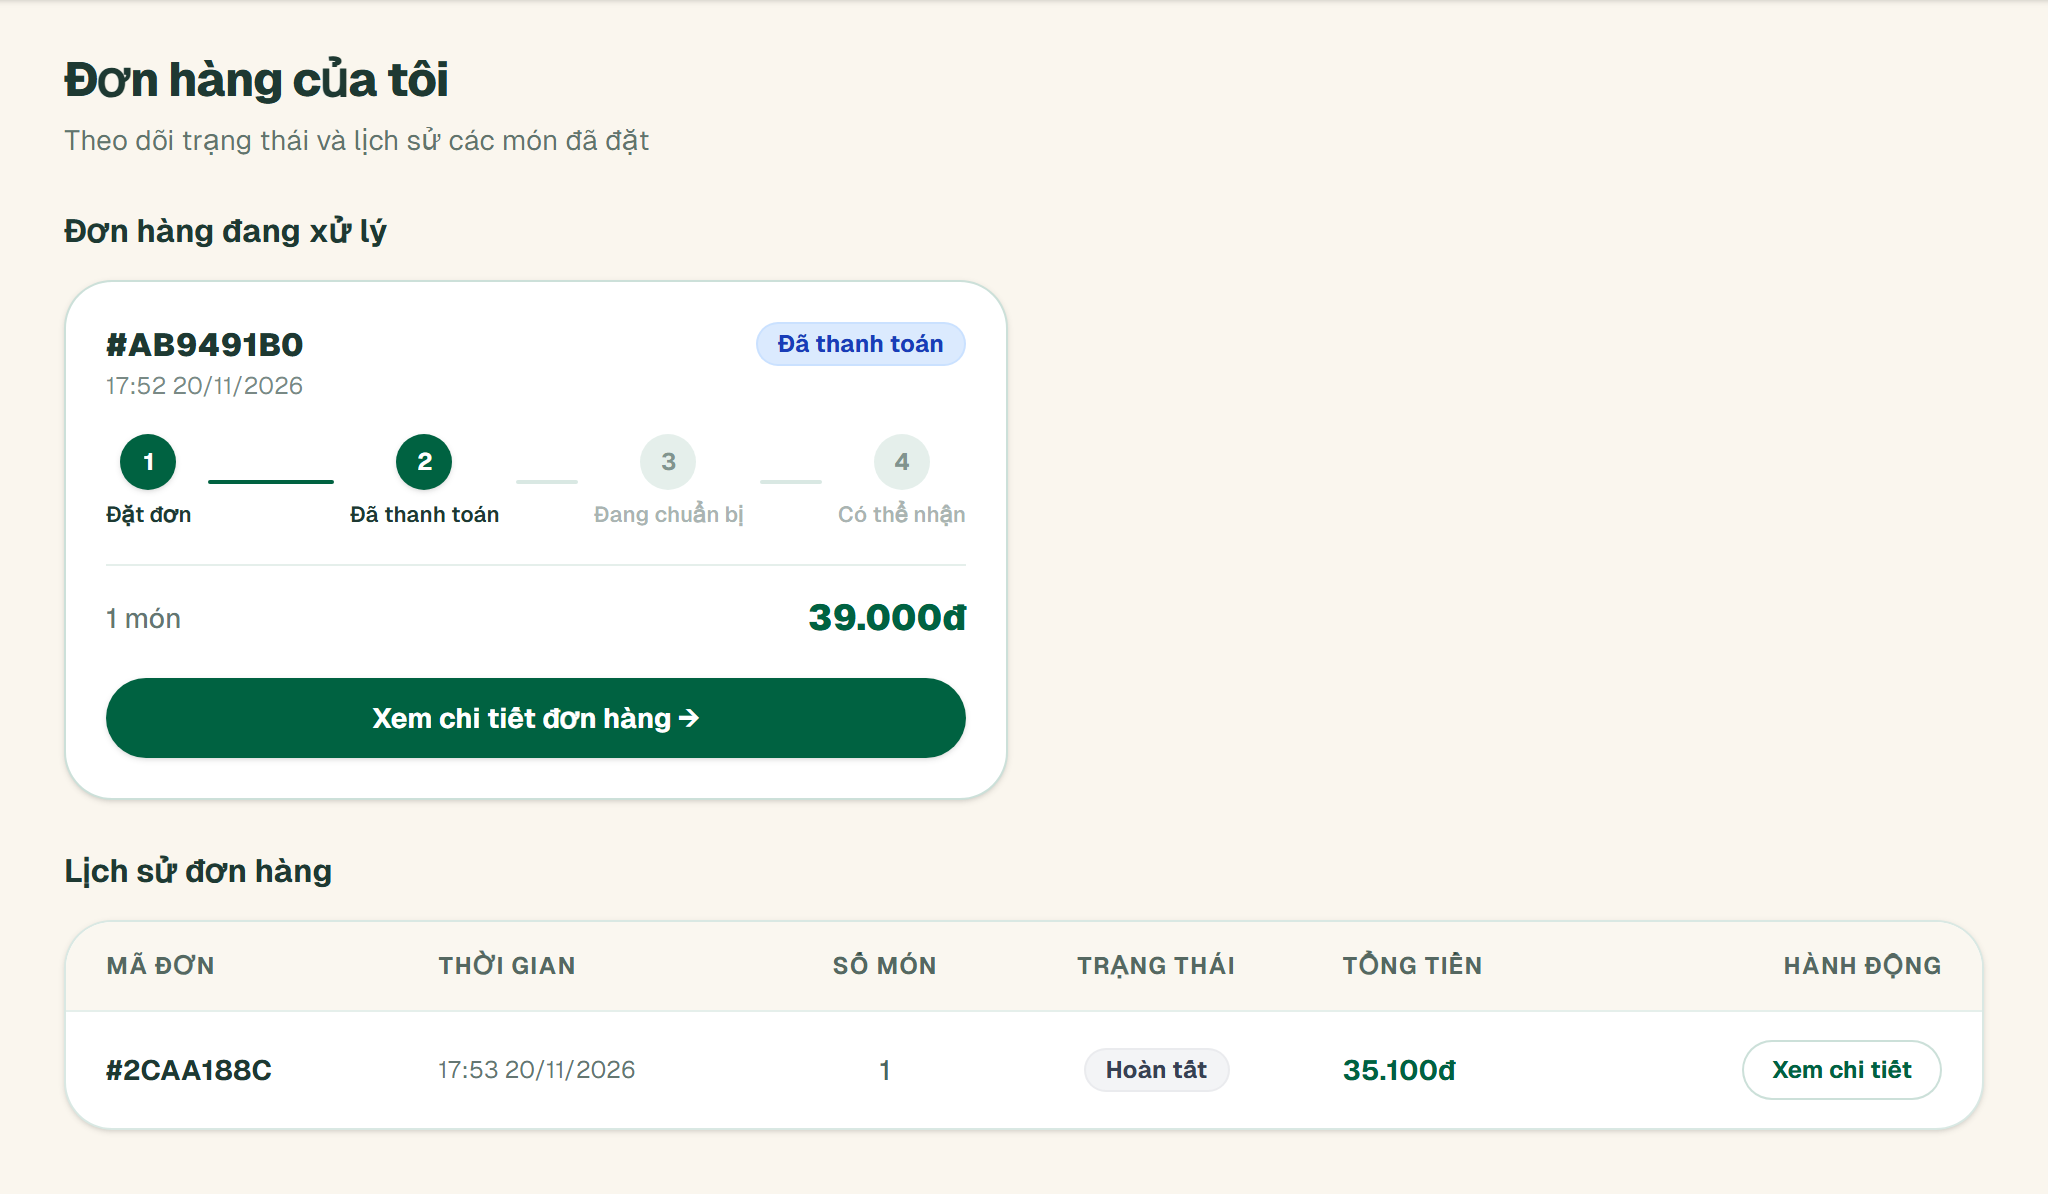
\includegraphics[width=\linewidth,height=.37\textheight,keepaspectratio]{../../assets/evidence/sprint2-history.png}
\par\small\itshape Hình 5.1e. Đơn demo xuất hiện trong lịch sử ở trạng thái Hoàn tất
\end{reportfigure}

Sau ảnh biên nhận, tài khoản ADMIN local chuyển đơn theo các bước
\texttt{PREPARING}, \texttt{READY}, \texttt{COMPLETED} để mô phỏng pha chế
và nhận đồ tại quầy. Ảnh lịch sử đối chiếu cùng đơn bắt đầu bằng
\texttt{2CAA188C}. Thông tin môi trường và mã đơn lưu trong tệp
\nolinkurl{sprint2-capture.json} tại thư mục \nolinkurl{docs/assets/evidence/}.
